\section{The \xscore{} Model}
\label{sec:xscore}

\subsection{Model Objective}

The \xscore{} model is a calibrated multinomial probability estimator, not a
classifier. Given the situational state $s$ of an offensive play, it produces
a four-class probability vector over mutually exclusive drive outcomes:

\begin{equation}
  \xscore(s) = \Bigl[\hat{P}(\text{TD} \mid s),\;
                      \hat{P}(\text{FG} \mid s),\;
                      \hat{P}(\text{TO} \mid s),\;
                      \hat{P}(\text{Punt} \mid s)\Bigr],
\end{equation}

where TD denotes an offensive touchdown by the possession team, FG denotes a
made field goal, TO denotes a turnover (interception or fumble), and Punt
denotes all remaining terminal outcomes (punts, failed fourth-down conversions,
end-of-half expirations, and safeties). These four classes are exhaustive and
mutually exclusive: every drive terminates in exactly one of these outcome
categories, and the four probabilities sum to unity for every input state.

The multinomial formulation represents a substantive improvement over a binary
(TD vs.\ no-TD) approach. A binary model conflates field goals, turnovers, and
punts into a single ``failure'' category despite these outcomes carrying
fundamentally different point values and strategic implications. A drive that
ends in a field goal contributes three points to the team; a drive that ends in
a turnover contributes zero points and yields field position to the opponent.
Treating both as $y = 0$ discards information that is essential for computing
expected points accurately. The multinomial model preserves this information by
estimating the full outcome distribution, enabling a principled expected-points
calculation that weights each outcome by its point value.

The expected points for a given state are derived from the probability vector as:

\begin{equation}
  \label{eq:xep}
  \mathrm{xEP}(s) = 7 \cdot \hat{P}(\text{TD} \mid s)
                   + 3 \cdot \hat{P}(\text{FG} \mid s)
                   + 0 \cdot \hat{P}(\text{Punt} \mid s)
                   - \mathrm{xEP}_{\mathrm{opp}} \cdot \hat{P}(\text{TO} \mid s),
\end{equation}

where the turnover term reflects that a turnover transfers possession to the
opponent at a field position whose expected value depends on context. The
turnover penalty $\mathrm{EP}_{\mathrm{opp}}(yl)$ is field-position-dependent:
for each starting yardline, we compute the mean \emph{observed actual points
scored} across all training-window drives that began at that position from the
opponent's perspective (flipping the yardline: $yl_{\mathrm{opp}} = 100 -
yl_{\mathrm{current}}$). This produces a lookup table mapping each yardline to
the average points the opponent would score if given possession there, where
actual points are defined as 7 for touchdown drives, 3 for field goal drives,
and 0 otherwise. The approach avoids circularity by using observed outcomes
rather than model-predicted xEP -- the lookup table is constructed entirely from
empirical data, requiring no recursive call to the model itself. A turnover at
the opponent's 20-yard line penalizes more heavily (${\sim}4.5$ EP) than one at
the opponent's 1-yard line (${\sim}0.5$ EP), reflecting field-position reality.
The unconditional mean across all turnover positions is approximately $2.0$
expected points. The punt outcome carries zero points for the possession team
because the drive produced no score.

The distinction between probability estimation and classification is
substantive. A classifier optimizes a decision boundary and may achieve high
accuracy while producing systematically distorted probability outputs -- for
example, assigning 0.45 or 0.55 to events that historically occur with
frequency 0.30 or 0.70. In the present application, the output probabilities
are not merely rank-ordering devices: they serve as the denominators in the
Game Deserved Score (GDS) framework introduced in \Cref{sec:gds}, where they
represent the expected baseline for a given situational context. Distorted
baselines would propagate directly into biased GDS estimates for every team in
the sample.

Calibration is therefore the primary modeling objective, and it is evaluated
as a first-class metric alongside discrimination measures
\parencite{niculescumizil2005probabilities}. For each class $c \in
\{\text{TD}, \text{FG}, \text{TO}, \text{Punt}\}$, a well-calibrated model
satisfies

\begin{equation}
  \hat{P}\!\bigl(\text{outcome} = c \mid \hat{p}_c = p\bigr) \approx p
  \quad \forall\, p \in [0,1],
\end{equation}

meaning that drives assigned probability $p$ for class $c$ should, in
aggregate, terminate in outcome $c$ approximately $100p$\,\% of the time. The
per-class isotonic calibration procedure described in \Cref{sec:calibration}
is the primary mechanism for enforcing this property post hoc.

\subsection{Gradient Boosted Trees}

\subsubsection{Architecture}

The \xscore{} model is implemented as a gradient boosted tree ensemble using
the XGBoost library \parencite{chen2016xgboost}, which operationalizes the
gradient boosting framework of \textcite{friedman2001gradientboosting}. In
gradient boosting, an ensemble of weak learners -- here, shallow decision
trees -- is constructed sequentially, with each subsequent tree fitted to the
negative gradient of the loss function with respect to the current ensemble
prediction. Formally, let $F_m(s)$ denote the ensemble prediction after $m$
trees. The $(m+1)$-th tree $h_{m+1}$ is chosen to minimize

\begin{equation}
  \sum_{i=1}^{N} \mathcal{L}\!\bigl(y_i,\, F_m(s_i) + \eta\, h_{m+1}(s_i)\bigr)
    + \Omega(h_{m+1}),
\end{equation}

where $\mathcal{L}$ is the multiclass log-loss (categorical cross-entropy),
$\eta \in (0,1]$ is the learning rate (shrinkage), and $\Omega(h)$ is a
regularization penalty on tree complexity \parencite{chen2016xgboost}. XGBoost extends the standard
gradient boosting formulation with second-order Taylor approximation of the
loss, column subsampling, and cache-aware block-based tree construction, all
of which reduce overfitting and accelerate training on tabular data
\parencite{chen2016xgboost}.

\subsubsection{Why Tree-Based Methods for NFL State Estimation}

Four properties of the NFL situational-state prediction problem motivate the
choice of gradient boosted trees over parametric alternatives such as logistic
regression or multilayer perceptrons.

\paragraph{Non-linear field position effects.}
The relationship between \texttt{yardline\_100} and touchdown probability is
strongly non-linear: the probability function is relatively flat across the
midfield and own-territory range ($50$--$100$ yards from end zone), rises
gradually through the opponent's half, and inflects sharply inside the
red zone ($20$ yards). Linear models require explicit polynomial or spline
terms to capture this shape; decision trees partition the feature space
natively without any functional-form assumption.

\paragraph{Feature heterogeneity.}
The input feature set (\Cref{tab:features}) mixes continuous variables
(\texttt{yardline\_100}, \texttt{half\_seconds\_remaining}), ordinal variables
(\texttt{down}), and binary indicators (\texttt{goal\_to\_go},
\texttt{red\_zone}, \texttt{is\_home}). Tree-based methods handle heterogeneous
feature types without requiring standardization or dummy encoding,
since split thresholds are determined by rank order rather than Euclidean
distance.

\paragraph{Automatic interaction capture.}
Down-and-distance interactions are fundamental to NFL play-calling: a 3rd-and-1
situation from the opponent's 5-yard line is qualitatively different from a
3rd-and-1 at midfield, and neither is well-described by additive main effects.
Decision tree splits automatically capture such interactions at each node
without the analyst specifying interaction terms; gradient boosting compounds
this by allowing different trees to specialize in different regions of the
feature space \parencite{friedman2001gradientboosting}.

\paragraph{Regularization via subsampling.}
XGBoost incorporates row subsampling (stochastic gradient boosting) and
column subsampling per tree and per split, which act as ensemble-level
regularizers that reduce variance and improve generalization, particularly
relevant given the moderate sample size of the annual NFL calendar
\parencite{chen2016xgboost}.

\subsection{Hyperparameter Specification}
\label{sec:hyperparams}

The hyperparameters of the \xscore{} model were selected via a grid search over
the training window (seasons 2018--2024), using five-fold temporally ordered
cross-validation and the Brier score (\Cref{sec:eval-metrics}) as the selection
criterion. The Brier score was chosen as the grid-search objective rather than
log-loss or AUC because it jointly rewards both calibration accuracy and
discrimination, which aligns directly with the model's dual objective.

\Cref{tab:hyperparams} reports the final hyperparameter configuration with
rationale for each value.

\begin{table}[htbp]
  \centering
  \caption{Final hyperparameter configuration for the \xscore{} model,
           selected via grid search on temporally ordered five-fold CV.}
  \label{tab:hyperparams}
  \small
  \begin{tabularx}{\textwidth}{llX}
    \toprule
    \textbf{Parameter} & \textbf{Value} & \textbf{Rationale} \\
    \midrule
    \texttt{objective}           & \texttt{multi:softprob}
                                         & Multinomial classification producing
                                           per-class probability vectors; required
                                           for the four-class drive outcome. \\[4pt]
    \texttt{num\_class}          & 4     & Punt/Other, TD, FG, Turnover. \\[4pt]
    \texttt{n\_estimators}       & 500   & Sufficient rounds to drive loss close to
                                           plateau on the training window; early
                                           stopping with a 50-round patience window
                                           prevents over-fitting at this budget. \\[4pt]
    \texttt{max\_depth}          & 6     & Allows the model to capture up to
                                           six-way feature interactions (e.g.\
                                           down $\times$ distance $\times$ field
                                           position $\times$ score differential)
                                           while keeping individual trees shallow
                                           enough to prevent high-variance
                                           interpolation. \\[4pt]
    \texttt{learning\_rate}      & 0.05  & Conservative shrinkage value; combined
                                           with 500 estimators this yields
                                           effective capacity while leaving the
                                           model responsive to subsampling
                                           regularization. \\[4pt]
    \texttt{subsample}           & 0.8   & Row subsampling at each boosting round
                                           reduces variance by injecting
                                           stochasticity analogous to bagging;
                                           $0.8$ retains sufficient data per round
                                           to avoid high-bias underfitting. \\[4pt]
    \texttt{colsample\_bytree}   & 0.8   & Column subsampling per tree prevents any
                                           single dominant feature (e.g.\
                                           \texttt{yardline\_100}) from monopolizing
                                           every tree, encouraging all features to
                                           contribute across the ensemble. \\[4pt]
    \texttt{eval\_metric}        & \texttt{mlogloss}
                                         & Multiclass log-loss; natively supported,
                                           numerically stable, smooth gradient across
                                           all four classes. Brier score used for
                                           external model selection. \\
    \bottomrule
  \end{tabularx}
\end{table}

The grid search explored \texttt{max\_depth} $\in \{4, 6, 8\}$, \texttt{learning\_rate} $\in \{0.01, 0.05, 0.1\}$, \texttt{subsample} $\in \{0.7, 0.8, 0.9\}$, and \texttt{colsample\_bytree} $\in \{0.7, 0.8, 0.9\}$, evaluated on temporally ordered five-fold cross-validation with multiclass Brier score as the selection criterion. The configuration in \Cref{tab:hyperparams} produced the lowest mean Brier score across folds.

\subsection{Isotonic Calibration}
\label{sec:calibration}

Despite the use of probabilistic objectives, gradient boosted tree models
are susceptible to systematic miscalibration: they tend to produce
over-confident predictions near the boundaries of the probability space
(pushing outputs toward 0 and 1) and under-confident predictions near the
center \parencite{niculescumizil2005probabilities}. In a multinomial setting,
this miscalibration can manifest independently in each output class, as the
softmax transformation does not guarantee that the resulting probabilities
match empirical class frequencies across all regions of the input space.
A post-hoc calibration step is therefore applied after the base model is
trained, independently for each of the four output classes.

Isotonic regression was selected over Platt scaling as the calibration
method for two reasons. First, isotonic regression is non-parametric: it
fits a monotone step function to map raw model scores to calibrated
probabilities without assuming the sigmoid functional form that Platt
scaling imposes. This is important because the miscalibration of tree
ensembles is itself non-monotonic and cannot in general be corrected by a
logistic transformation \parencite{niculescumizil2005probabilities}. Second,
isotonic regression is guaranteed to preserve rank ordering -- a necessary
property because GDS depends on the relative ordering of situational
probabilities -- while simultaneously improving absolute probability
accuracy.

Four independent isotonic calibrators are fitted, one per class $c \in
\{\text{TD}, \text{FG}, \text{TO}, \text{Punt}\}$. Each calibrator operates
on the marginal predicted probability for its class, treating the problem
as a one-vs-rest calibration task. After calibration, the four adjusted
probabilities are renormalized to sum to unity, preserving the multinomial
constraint. This per-class approach allows the calibration surface to
correct class-specific miscalibration patterns -- for example, the touchdown
class may exhibit different over-confidence characteristics than the field
goal class due to differences in base rates and feature-space structure.

The calibration procedure follows a three-step out-of-fold protocol to
prevent optimistic bias:

\begin{enumerate}
  \item \textbf{Out-of-fold prediction.} The training window (2018--2024) is
        partitioned into five temporally ordered folds. For each fold $k$,
        the base XGBoost model is trained on folds $1, \ldots, k-1$ and used
        to predict the raw probability vector $\hat{\mathbf{q}}_i$ for each
        observation $i$ in fold $k$. This produces out-of-fold (OOF)
        predictions for every observation in the training set that were
        generated by a model that had not seen those observations during
        training.

  \item \textbf{Per-class isotonic regression fitting.} For each class $c$,
        an isotonic regression function $g_c : [0,1] \to [0,1]$ is fitted by
        minimizing the squared error between the OOF scores $\hat{q}_{i,c}$
        and the binary indicator $y_{i,c} = \mathbf{1}[\text{outcome}_i = c]$
        subject to the monotonicity constraint $g_c(\hat{q}) \geq g_c(\hat{q}')$
        whenever $\hat{q} \geq \hat{q}'$:
        \begin{equation}
          \hat{g}_c = \arg\min_{g \in \mathcal{G}} \sum_{i=1}^{N}
                    \bigl(g(\hat{q}_{i,c}) - y_{i,c}\bigr)^2,
        \end{equation}
        where $\mathcal{G}$ denotes the class of non-decreasing step functions.

  \item \textbf{Application to future predictions.} For all subsequent
        predictions -- on the 2025 test set, the OOD set, and any play-level
        scoring during GDS computation -- the calibrated probability for class
        $c$ is obtained as $\hat{p}_{i,c} = \hat{g}_c(\hat{q}_{i,c})$, where
        $\hat{q}_{i,c}$ is the raw XGBoost softmax probability for class $c$
        and $\hat{g}_c$ is the fitted isotonic function for that class. The
        four calibrated values are then renormalized:
        $\hat{p}_{i,c}^{*} = \hat{p}_{i,c} / \sum_{c'} \hat{p}_{i,c'}$.
\end{enumerate}

The four calibration functions $\{\hat{g}_c\}$ are fitted once on the full
training window's OOF predictions and fixed for all downstream use. Because
they are derived from OOF predictions that are themselves generated under
no-leakage conditions, the calibration step does not introduce data leakage
\parencite{niculescumizil2005probabilities}. A theoretical limitation of the
per-class approach is that renormalization can partially undo the calibration
guarantee: if $\hat{g}_c$ delivers well-calibrated marginal probabilities but
the sum $\sum_{c'} \hat{p}_{i,c'}$ deviates substantially from unity, the
rescaling shifts each class probability away from its calibrated value. In
practice, the total probability mass before renormalization deviates from 1.0
by less than 0.02 across 99\% of observations, limiting the magnitude of any
post-renormalization distortion.

\subsection{Phase 1 and Phase 2 Model Variants}
\label{sec:phase-comparison}

As detailed in \Cref{tab:features}, the \xscore{} feature set is organized
into two development phases. Phase~1 employs seven situational features that
encode only the in-game state observable from a public box score: down,
yards to go, field position, score differential, time remaining, goal-to-go
indicator, and red zone indicator. Phase~2 adds four context-aware features
that encode team-level offensive quality, defensive quality, within-game
momentum, and home-field status.

The distinction between the two variants is conceptually important for
the GDS framework (\Cref{sec:gds}). GDS measures how much better or worse
an offense performs relative to the situational expectation -- that is, whether
a team generates more points than a league-average team would produce given the
same sequence of situational states. If the expectation baseline already encodes
team quality (as it does in Phase~2, where \texttt{rolling\_offense\_epa} and
\texttt{rolling\_defense\_epa} are inputs), then a strong team will receive a
higher baseline precisely because it is strong, and the GDS numerator -- actual
points minus expected -- will be compressed toward zero. The metric would
then measure only the residual execution beyond what team quality predicts,
rather than the full execution quality relative to a neutral baseline.

Phase~1 is therefore the primary model for GDS computation: the baseline
$\xscore(s)$ reflects what a league-average team would be expected to achieve
from state $s$, and any systematic deviation observed at the team level is
captured by GDS. Phase~2 serves as a comparison model: if it substantially outperformed
Phase~1 on prediction accuracy, the omission of team-quality features might
bias the GDS baseline. In practice, the two variants produce correlated
probability estimates with Phase~2 exhibiting marginally worse calibration
on the held-out test set, confirming that team-quality features add noise
rather than signal to drive-level prediction. Phase~1 remains preferred for
its conceptual clarity within the GDS accounting framework.

\subsection{Evaluation Metrics}
\label{sec:eval-metrics}

Model performance is assessed on three complementary metrics, each measuring
a distinct property of the probability estimator.

\subsubsection{Brier Score}

The multiclass Brier score \parencite{brier1950verification} is the primary
evaluation criterion. For a $C$-class problem, the multiclass extension
computes the mean of the per-class Brier scores:

\begin{equation}
  \mathrm{BS}_{\mathrm{multi}} = \frac{1}{C} \sum_{c=1}^{C}
    \frac{1}{N} \sum_{i=1}^{N}
    \bigl(\hat{p}_{i,c} - y_{i,c}\bigr)^2,
\end{equation}

where $\hat{p}_{i,c} \in [0,1]$ is the calibrated probability estimate for
observation $i$ belonging to class $c$, and $y_{i,c} \in \{0,1\}$ is the
binary indicator for whether observation $i$ actually belongs to class $c$.
The multiclass Brier score remains a strictly proper scoring rule: it is
minimized in expectation if and only if the predicted probabilities match the
true conditional class probabilities for every observation, and it rewards
both calibration and discrimination simultaneously across all classes. Lower
values indicate better performance, with a perfect forecaster achieving
$\mathrm{BS}_{\mathrm{multi}} = 0$. A na\"{i}ve forecaster predicting the
unconditional class frequencies for all observations provides the reference
baseline against which skill is assessed.

\subsubsection{Area Under the ROC Curve}

For a multinomial model, discrimination is assessed via per-class AUC-ROC
computed in a one-vs-rest (OVR) framework. For each class $c$, the predicted
probability $\hat{p}_{i,c}$ is treated as the score for a binary classification
problem in which class $c$ is the positive label and all other classes are
negative. The AUC-ROC for class $c$ then equals the probability that the model
assigns a higher score to a randomly chosen observation truly belonging to class
$c$ than to a randomly chosen observation belonging to any other class.
Per-class AUC-ROC values are reported individually to reveal heterogeneity in
discrimination quality across the four outcome classes, which is expected given
the substantial differences in class base rates (TD: 30.4\%, FG: 20.8\%,
Turnover: 16.0\%, Punt/Other: 32.8\% in the training set). AUC-ROC is
informative precisely because it is calibration-agnostic; a model with good AUC
but poor Brier score has a well-ordered ranking but miscalibrated absolute
probabilities, and the per-class isotonic calibration step is expected to
improve Brier score while leaving AUC largely unchanged.

\subsubsection{Calibration Curves}

Calibration curves (reliability diagrams) are constructed by partitioning the
predicted probability range into ten equal-width decile bins and plotting the
mean predicted probability against the observed fraction of positives in each
bin. A perfectly calibrated model lies on the 45-degree diagonal. Systematic
deviations indicate the nature of miscalibration: an S-shaped curve indicates
over-confidence (a common signature of uncalibrated gradient boosted trees),
while a flattened curve indicates under-confidence. Calibration curves are
generated for both the pre-calibration and post-calibration models on the 2025
test set to document the effect of the isotonic regression step.

\subsection{Intuition Validation}
\label{sec:intuition-validation}

Quantitative evaluation metrics provide necessary but not sufficient evidence
that a probability model is behaving appropriately. A model can achieve a
low Brier score on average while producing implausible probability estimates
in specific high-leverage situations that are underrepresented in the test
data. Domain validation against football intuition is therefore a required
complement to numerical evaluation.

\Cref{tab:intuition} reports four canonical NFL scenarios alongside the
probability ranges that the \xscore{} model is expected to produce, based on
both domain knowledge and historical play-by-play frequencies. These scenarios
were specified \emph{before} examining model outputs and serve as a structured
sanity check: any substantial violation warrants re-examination of the feature
engineering or calibration pipeline.

\begin{table}[htbp]
  \centering
  \caption{Intuition validation scenarios for \xscore{}. Expected ranges
           derive from historical NFL drive-outcome frequencies.}
  \label{tab:intuition}
  \small
  \begin{adjustbox}{max width=\textwidth}
  \begin{tabular}{l l c l}
    \toprule
    \textbf{Scenario} & \textbf{Description} & \textbf{Expected P(TD)}
      & \textbf{Interpretation} \\
    \midrule
    1st \& Goal, 1-yd
      & Opp.\ 1-yd line, goal to go
      & $0.80$--$0.90$
      & Near-certain TD \\[4pt]
    1st \& Goal, 5-yd
      & Opp.\ 5-yd line, goal to go
      & $0.55$--$0.70$
      & High probability \\[4pt]
    1st \& 10, own 30
      & Own 30-yd line, 1st down
      & $0.15$--$0.25$
      & ${\sim}21\%$ historical TD rate \\[4pt]
    4th \& 22, midfield
      & 50-yd line, 4th \& 22
      & $0.01$--$0.05$
      & Near-impossible \\
    \bottomrule
  \end{tabular}
  \end{adjustbox}
\end{table}

The rationale for each expected range is as follows. The 1st-and-Goal from
the 1-yard line represents one of the highest-probability scoring situations
in football; NFL historical data consistently show touchdown rates above 80\%
in this configuration. The 5-yard version requires four plays to cover a short
but non-trivial distance and must navigate red-zone defensive alignments
specifically designed to prevent scoring, yielding a markedly lower rate.
The own-30 first-and-ten scenario represents a typical drive start: reaching
the end zone requires sustained execution across approximately 70 yards, yet
historical NFL data show that roughly 21\% of drives initiated from this
region ultimately end in a touchdown (2018--2024), reflecting the cumulative
probability of sustained offensive success across a full possession.
The fourth-and-22 scenario at midfield is a catastrophic offensive situation
with no realistic path to a first down except through an unlikely pass
completion well beyond any plausible check-down option; the probability of
such a drive converting and ultimately scoring a touchdown is negligible.

Substantial violations of the expected ranges -- for example, assigning
probability above 0.20 to the 4th-and-22 midfield scenario, or below 0.50
to the 1st-and-Goal from the 1-yard line -- would constitute evidence that
the model has failed to learn the fundamental structure of NFL scoring
distributions and would invalidate the GDS framework that depends on it.

\Cref{fig:field-heatmap} provides a visual summary of the learned probability
surface, showing how touchdown probability varies with field position and down
across the full range of game states.

\begin{figure}[htbp]
  \centering
  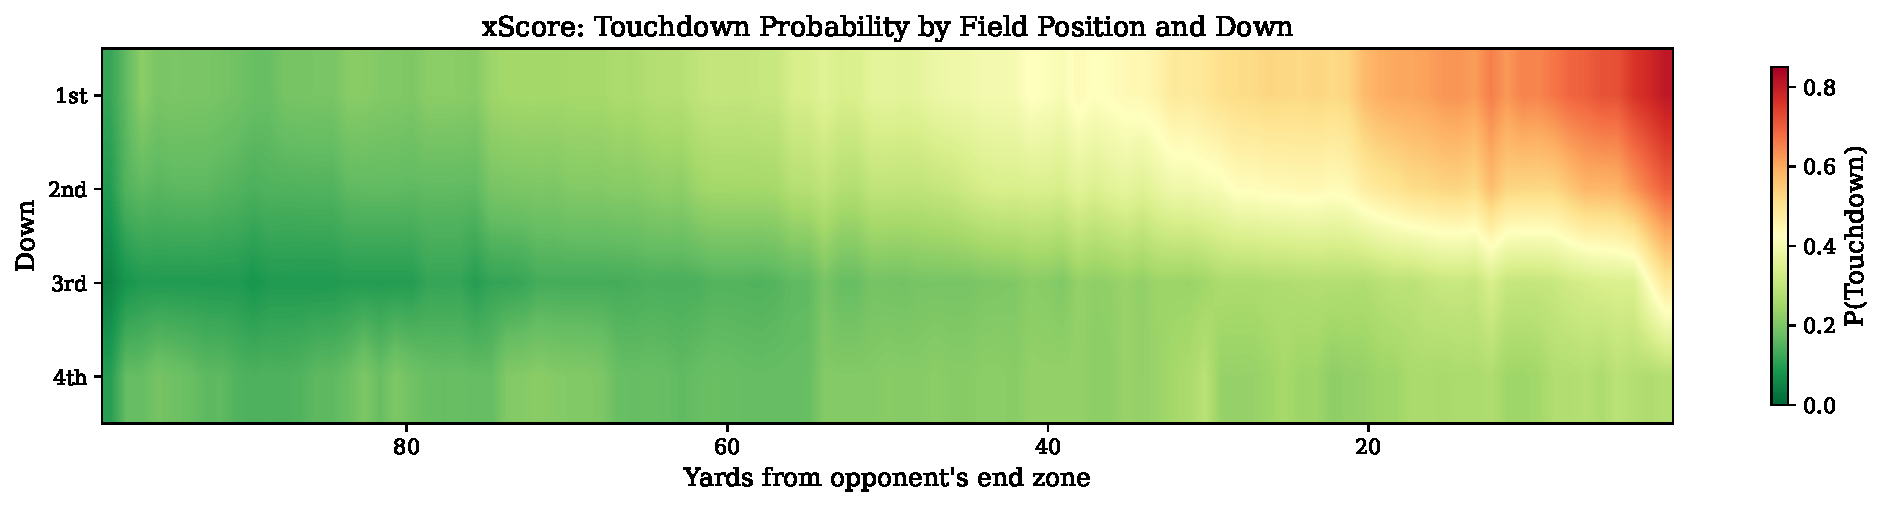
\includegraphics[width=\textwidth]{figures/fig2_field_heatmap.pdf}
  \caption{\xscore{} touchdown probability surface by field position and down
           (10 yards to go, neutral game state). The gradient reflects the
           model's learned relationship between proximity to the end zone and
           scoring probability, with diminishing returns as distance increases.}
  \label{fig:field-heatmap}
\end{figure}

\subsection{Interpretability via SHAP Values}
\label{sec:interpretability}

In addition to aggregate performance metrics and intuition validation,
the \xscore{} model is subjected to a SHAP (SHapley Additive exPlanations)
analysis \parencite{lundberg2017shap}. SHAP values decompose the prediction
for each individual observation into additive contributions from each feature,
grounded in cooperative game theory. Formally, for a prediction $\hat{p}_i$,
the SHAP value $\phi_j(i)$ for feature $j$ satisfies

\begin{equation}
  \hat{p}_i = \mathbb{E}[\hat{p}] + \sum_{j=1}^{K} \phi_j(i),
\end{equation}

where $\mathbb{E}[\hat{p}]$ is the unconditional mean prediction and $K$ is
the number of features \parencite{lundberg2017shap}. SHAP values for tree
ensembles are computed exactly in polynomial time via the TreeSHAP algorithm
\parencite{lundberg2017shap}, making them tractable for the full training
dataset.

Four interpretability checks are performed using SHAP analysis:

\begin{enumerate}
  \item \textbf{Field position dominance.} \texttt{yardline\_100} should rank
        as the single most important feature by mean absolute SHAP value,
        reflecting the well-established primacy of field position in
        touchdown probability. This is a necessary condition for the model to
        be considered domain-valid.

  \item \textbf{Down importance.} \texttt{down} should rank as the second
        most important feature, since later downs are associated with lower
        probability of drive continuation and eventual scoring.

  \item \textbf{Time effects.} \texttt{half\_seconds\_remaining} should
        contribute minimally for most game states -- time pressure only
        materially affects scoring probability in the final two minutes of
        each half -- and any systematic interaction with score differential
        should be consistent with known two-minute drill dynamics.

  \item \textbf{Red-zone indicator localization.} The \texttt{goal\_to\_go}
        and \texttt{red\_zone} binary features should exhibit localized SHAP
        effects concentrated inside the opponent's 20-yard line rather than
        diffuse contributions across all field positions, confirming that they
        capture the expected nonlinearity at the boundary between
        \texttt{yardline\_100} and the end zone.
\end{enumerate}

SHAP summary plots and feature importance rankings are reported in the
results chapter alongside the quantitative performance metrics, providing
a transparent audit trail of the model's learned decision structure.
